\chapter{Misc}\label{chap:misc}
\section{Solution to the Chessboard Problem}
\begin{sproof}[Solution]\label{sol:chessboard}
  \textbf{Claim:} No.\\

  \noindent \emph{Proof:} {Observe that there} are {25 black squares}
  and {24 white squares}. {Also} {note that every legal move takes} a
  {knight to} an {opposite-color square}. {Hence} {after moving all}
  the {knights}, {we}'{d have 25 on black} and {24 on white}, {which
    is} a {contradiction}. \hfill {$\jiong$}
  \renewcommand{\qed}{}
\end{sproof}
\section{\texttt{Julia} Code for the Countable Reidemeister I
  Example}\label{sec:Julia-for-countable-reidemeister-i}
\begin{lstlisting}
using Plots
using Colors
plotlyjs()

# r₁ is the big r for the circle this is based on.
#
# This function just computes the equation seen in our explicit
# parameterization of the countable reidemeister I knot. Note that
# this uses the form defined in terms of the matrix-vector equation,
# since we found it more tangible when prototyping.
function to_cartesian(θ; r₁=3)
    # This is the special "f(0)=0" case in our piecewise definition of
    # our function.
    if θ == 0
        return [r₁,0,0]
    end

    # Compute the radius of the smaller circle
    r₂ = abs(θ)^3
    x = r₁*cos(θ)
    y = r₁*sin(θ)

    # The radial vector is orthogonal to the tangent vector, hence
    # we can use it as one of the basis vectors for the orthogonal
    # frame.
    vperp = [x, y, 0]
    vperp /= sqrt((x^2 + y^2)) # Normalize it

    # Since the big circle lies in the xy-plane, the z direction is
    # also always one of the basis vectors for the orthogonal plane.
    zperp = [0,0,1]

    scale=2*π^2
    if θ > 0
        v_to_transform = [r₂*sin(scale/θ), r₂*cos(scale/θ), 0.0]
    else
        v_to_transform = [r₂*sin(-1*scale/θ), r₂*cos(scale/θ), 0.0]
    end

    # Rotate into the orthogonal plane
    R_mat = [zperp vperp [0.0; 0.0; 0.0]]
    v_out = (R_mat * v_to_transform) + [x,y,0]
    return v_out
end

step = .0001
θs = 0:step:π/2
θ₂s = reverse(-1 .* θs)


xyz_vals = to_cartesian.(θs)
xyz_opp = to_cartesian.(θ₂s) # The mirror image
append!(xyz_opp, xyz_vals)

xs = [p[1] for p in xyz_opp]
ys = [p[2] for p in xyz_opp]
zs = [p[3] for p in xyz_opp]

lcol= colorant"#D6D7D9"
bcol= colorant"#1D252C"

plot(camera=(60, 25), size=(1500,1000),
     legend=false, background_color=bcol,
     color = lcol)#, grid=false)#, axis=false, ticks=false)

plot!(xs, ys, zs, color=lcol, lw=.5)
\end{lstlisting}

\section{Combinatorial Representations}\label{app:combinatorial-representations}
\subsection{Cycle representations}
\begin{table}[H]
  \centering
  \small
  \begin{tabular}{clc}
    \toprule
    Index & Cycle representation & Order \\ \midrule
    $(3, 1)$ & $(-3, -2) (1, 2)$ & 2 \\
$(4, 1)$ & $(-3, -2i, 4, 3, i, -i, 2i)$ & 7 \\
$(5, 1)$ & $(-5, -4, -2, -3) (1, 2, 4, 3)$ & 4 \\
$(5, 2)$ & $(-5, -4, -2, -3) (1, 2, 4)$ & 12 \\
$(6, 1)$ & $(-2, -3i, 6i, -4i, 1, 2, 4i) (-6i, 3i, -5i, 5i)$ & 28 \\
$(6, 2)$ & $(-6, -2i, 4i) (-5i, 5i, -4i, 3i) (-3i, 1, 2i)$ & 12 \\
$(6, 3)$ & $(-6, 4i, 6) (-5, 5, -3i) (-1, 1, -2i, -4i) (2i, 3i)$ & 12 \\
$(6, 4)$ & $(-6, -5) (-3, -2) (1, 2) (4, 5)$ & 2 \\
$(6, 5)$ & $(-3, -2) (-5i, -4i) (5i, 6i) (1, 2)$ & 2 \\
$(7, 1)$ & $(-7, -6, -4) (-5, -2, -3) (1, 2, 4) (3, 6, 5)$ & 3 \\
$(7, 2)$ & $(-7i, 2i) (-6i, 4i, -4i, 5i) (-5i, 7i, -3i, 3i, -2i, i, -i, 6i)$ & 8 \\
$(7, 3)$ & $(-7, -6, -4, -5, -2, -3) (1, 2, 4) (3, 6, 5)$ & 6 \\
$(7, 4)$ & $(-7, -6, -2, -3, -5, -4) (1, 2, 4) (3, 6, 7, 5)$ & 12 \\
$(7, 5)$ & $(-7i, 6i, -4i, 3i, -5i, 7i) (-6i, 5i) (-3i, i, -i, 2i) (-2i, 4i)$ & 12 \\
$(7, 6)$ & $(-3, -5i, i, -i, 2i) (-7i, 7i, -2i, 4, 3, 6i, -6i, 5i)$ & 40 \\
$(7, 7)$ & $(-6, -4) (-3, -2i, 4, 7, 6, 3, 5i, -5i, i, -i, 2i)$ & 22 \\
$(8, 1)$ & $(-4, -5i, 8i, -6i, 3, i, -i, 2i, -3, -2i, 4, 6i) (-8i, 5i, -7i, 7i)$ & 12 \\
$(8, 2)$ & $(-2, 3i, 5i, 2, -4i, -8i, -7i, -5i, -1, 1) (-6i, -3i) (4i, 7i) (6i, 8i)$ & 10 \\
$(8, 3)$ & $(-4, -7i, 7i, -8i, 5i) (-3, -5i, 3, 6i, -2) (-6i, 1, 2, 4, 8i)$ & 5 \\
$(8, 4)$ & $(-5, -8i, 8i, -7i, 6i, -4, -6i, 3, i, -i, 2, 4, 7i, -2, -3)$ & 15 \\
$(8, 5)$ & $(-8, -4, -7) (-5, -2i, 4, 8, 5, i, -i, 2i, -3) (3, 6, 7)$ & 9 \\
$(8, 6)$ & $(-2, 3i, 5i, 2, -4i, -8i, -5i, -1, 1) (-7i, -3i, -6i) (4i, 7i, 6i, 8i)$ & 36 \\
$(8, 7)$ & $(-8, -7, -5) (-6, -2i, i, -i, 2i, -3i, 5, 4, 7, 6, 3i, -4)$ & 12 \\
$(8, 8)$ & $(-8, 7, -1, 1, -2, 3, -6i, -3, 5i, 8) (-7, 2, -4i)$ & 30 \\
$(8, 9)$ & $(-8, -6, -4i, 8, 7, 5, 3i, -5, -2i, 4i, -7) (-3i, 6, i, -i, 2i)$ & 55 \\
$(8, 10)$ & $(-5, -7i, 7i, -6i, 8i, -8i, 5, 3, 1, 2, 4, 6i, -4, -2, -3)$ & 15 \\
$(8, 11)$ & $(-2, 3i, 5i, 2, -4i, -8i, -7i, -3i, -6i, -5i, -1, 1) (4i, 7i) (6i, 8i)$ & 12 \\
$(8, 12)$ & $(-3, -5i, 8i, -6i, 1, 2, 4, 3, 6i, -2) (-8i, 5i, -7i, 7i)$ & 20 \\
$(8, 13)$ & $(-7, 4, -3, 5, -i, -2i, -4, 7) (-6, 2i, 3) (-5, 8i, 6, -8i)$ & 24 \\
$(8, 14)$ & $(-2, -3i, 6i) (-8i, 3i, -5i, 8i) (-7i, 7i, -6i, 1, 2, 4i) (-4i, 5i)$ & 12 \\
$(8, 15)$ & $(-8i, -5i, -6i, -i, -2i, -4i, -7i) (2i, 3i, 5i, 8i, 4i, 6i)$ & 42 \\
$(8, 16)$ & $(-6, 8i, 6, -i, -2, 3) (-3, 5i, 4i, 2, -4i, -7i)$ & 6 \\
$(8, 17)$ & $(-6, -8i, 8i, -7i, 3, 6, i, -i, 2i, -3, -5, -4, -2i, 4, 7i)$ & 15 \\
$(8, 18)$ & $(-5, -4, -2i, 4, 7, 3i) (-8i, 5, 8i) (-6i, 1, 2i, -3i, 6i)$ & 30 \\
$(8, 19)$ & $(-8, -7, 6, -5, 4, -6) (-4, -2, -3, 5, 7, 3, 1, 2)$ & 24 \\
$(8, 20)$ & $(-4, 6i, 8i, 7i, -2i) (-3, -5i, -7i, -6i, 5i, 4) (2i, 3, 1)$ & 30 \\
$(8, 21)$ & $(-6, 8i, 6, 7i, -2i, -4i, 1, 2i, -3i) (-7i, 3i, 5i, 4i)$ & 36 \\

    \bottomrule
  \end{tabular}
  \caption[Cycle presentations]{$\ms N_{\rm g.int}$ cycle
    presentations for knots up to $8$ crossings}
  \label{tab:cycle-gint}
\end{table}

\begin{table}[H]
  \centering
  \small
  \begin{tabular}{clc}
    \toprule
    Index & Cycle representation & Order \\ \midrule
    $(3, 1)$ & $(3^+_u, 2^+_u)(1^+_o, 2^+_o)$ & 2 \\
$(4, 1)$ & $(3^+_u, 2^-_u, 4^+_o, 3^+_o, 1^-_o, 1^-_u, 2^-_o)$ & 7 \\
$(5, 1)$ & $(5^+_u, 4^+_u, 2^+_u, 3^+_u)(1^+_o, 2^+_o, 4^+_o, 3^+_o)$ & 4 \\
$(5, 2)$ & $(5^+_u, 4^+_u, 2^+_u, 3^+_u)(1^+_o, 2^+_o, 4^+_o)$ & 12 \\
$(6, 1)$ & $(2^+_u, 3^-_u, 6^-_o, 4^-_u, 1^+_o, 2^+_o, 4^-_o)(6^-_u, 3^-_o, 5^-_u, 5^-_o)$ & 28 \\
$(6, 2)$ & $(6^+_u, 2^-_u, 4^-_o)(5^-_u, 5^-_o, 4^-_u, 3^-_o)(3^-_u, 1^+_o, 2^-_o)$ & 12 \\
$(6, 3)$ & $(6^+_u, 4^-_o, 6^+_o)(5^+_u, 5^+_o, 3^-_u)(1^+_u, 1^+_o, 2^-_u, 4^-_u)(2^-_o, 3^-_o)$ & 12 \\
$(6, 4)$ & $(6^+_u, 5^+_u)(3^+_u, 2^+_u)(1^+_o, 2^+_o)(4^+_o, 5^+_o)$ & 2 \\
$(6, 5)$ & $(3^+_u, 2^+_u)(5^-_u, 4^-_u)(5^-_o, 6^-_o)(1^+_o, 2^+_o)$ & 2 \\
$(7, 1)$ & $(7^+_u, 6^+_u, 4^+_u)(5^+_u, 2^+_u, 3^+_u)(1^+_o, 2^+_o, 4^+_o)(3^+_o, 6^+_o, 5^+_o)$ & 3 \\
$(7, 2)$ & $(7^-_u, 2^-_o)(6^-_u, 4^-_o, 4^-_u, 5^-_o)(5^-_u, 7^-_o, 3^-_u, 3^-_o, 2^-_u, 1^-_o, 1^-_u, 6^-_o)$ & 8 \\
$(7, 3)$ & $(7^+_u, 6^+_u, 4^+_u, 5^+_u, 2^+_u, 3^+_u)(1^+_o, 2^+_o, 4^+_o)(3^+_o, 6^+_o, 5^+_o)$ & 6 \\
$(7, 4)$ & $(7^+_u, 6^+_u, 2^+_u, 3^+_u, 5^+_u, 4^+_u)(1^+_o, 2^+_o, 4^+_o)(3^+_o, 6^+_o, 7^+_o, 5^+_o)$ & 12 \\
$(7, 5)$ & $(7^-_u, 6^-_o, 4^-_u, 3^-_o, 5^-_u, 7^-_o)(6^-_u, 5^-_o)(3^-_u, 1^-_o, 1^-_u, 2^-_o)(2^-_u, 4^-_o)$ & 12 \\
$(7, 6)$ & $(3^+_u, 5^-_u, 1^-_o, 1^-_u, 2^-_o)(7^-_u, 7^-_o, 2^-_u, 4^+_o, 3^+_o, 6^-_o, 6^-_u, 5^-_o)$ & 40 \\
$(7, 7)$ & $(6^+_u, 4^+_u)(3^+_u, 2^-_u, 4^+_o, 7^+_o, 6^+_o, 3^+_o, 5^-_o, 5^-_u, 1^-_o, 1^-_u, 2^-_o)$ & 22 \\
$(8, 1)$ & $(4^+_u, 5^-_u, 8^-_o, 6^-_u, 3^+_o, 1^-_o, 1^-_u, 2^-_o, 3^+_u, 2^-_u, 4^+_o, 6^-_o)(8^-_u, 5^-_o, 7^-_u, 7^-_o)$ & 12 \\
$(8, 2)$ & $(2^+_u, 3^-_o, 5^-_o, 2^+_o, 4^-_u, 8^-_u, 7^-_u, 5^-_u, 1^+_u, 1^+_o)(6^-_u, 3^-_u)(4^-_o, 7^-_o)(6^-_o, 8^-_o)$ & 10 \\
$(8, 3)$ & $(4^+_u, 7^-_u, 7^-_o, 8^-_u, 5^-_o)(3^+_u, 5^-_u, 3^+_o, 6^-_o, 2^+_u)(6^-_u, 1^+_o, 2^+_o, 4^+_o, 8^-_o)$ & 5 \\
$(8, 4)$ & $(5^+_u, 8^-_u, 8^-_o, 7^-_u, 6^-_o, 4^+_u, 6^-_u, 3^+_o, 1^-_o, 1^-_u, 2^+_o, 4^+_o, 7^-_o, 2^+_u, 3^+_u)$ & 15 \\
$(8, 5)$ & $(8^+_u, 4^+_u, 7^+_u)(5^+_u, 2^-_u, 4^+_o, 8^+_o, 5^+_o, 1^-_o, 1^-_u, 2^-_o, 3^+_u)(3^+_o, 6^+_o, 7^+_o)$ & 9 \\
$(8, 6)$ & $(2^+_u, 3^-_o, 5^-_o, 2^+_o, 4^-_u, 8^-_u, 5^-_u, 1^+_u, 1^+_o)(7^-_u, 3^-_u, 6^-_u)(4^-_o, 7^-_o, 6^-_o, 8^-_o)$ & 36 \\
$(8, 7)$ & $(8^+_u, 7^+_u, 5^+_u)(6^+_u, 2^-_u, 1^-_o, 1^-_u, 2^-_o, 3^-_u, 5^+_o, 4^+_o, 7^+_o, 6^+_o, 3^-_o, 4^+_u)$ & 12 \\
$(8, 8)$ & $(8^+_u, 7^+_o, 1^+_u, 1^+_o, 2^+_u, 3^+_o, 6^-_u, 3^+_u, 5^-_o, 8^+_o)(7^+_u, 2^+_o, 4^-_u)$ & 30 \\
$(8, 9)$ & $(8^+_u, 6^+_u, 4^-_u, 8^+_o, 7^+_o, 5^+_o, 3^-_o, 5^+_u, 2^-_u, 4^-_o, 7^+_u)(3^-_u, 6^+_o, 1^-_o, 1^-_u, 2^-_o)$ & 55 \\
$(8, 10)$ & $(5^+_u, 7^-_u, 7^-_o, 6^-_u, 8^-_o, 8^-_u, 5^+_o, 3^+_o, 1^+_o, 2^+_o, 4^+_o, 6^-_o, 4^+_u, 2^+_u, 3^+_u)$ & 15 \\
$(8, 11)$ & $(2^+_u, 3^-_o, 5^-_o, 2^+_o, 4^-_u, 8^-_u, 7^-_u, 3^-_u, 6^-_u, 5^-_u, 1^+_u, 1^+_o)(4^-_o, 7^-_o)(6^-_o, 8^-_o)$ & 12 \\
$(8, 12)$ & $(3^+_u, 5^-_u, 8^-_o, 6^-_u, 1^+_o, 2^+_o, 4^+_o, 3^+_o, 6^-_o, 2^+_u)(8^-_u, 5^-_o, 7^-_u, 7^-_o)$ & 20 \\
$(8, 13)$ & $(7^+_u, 4^+_o, 3^+_u, 5^+_o, 1^-_u, 2^-_u, 4^+_u, 7^+_o)(6^+_u, 2^-_o, 3^+_o)(5^+_u, 8^-_o, 6^+_o, 8^-_u)$ & 24 \\
$(8, 14)$ & $(2^+_u, 3^-_u, 6^-_o)(8^-_u, 3^-_o, 5^-_u, 8^-_o)(7^-_u, 7^-_o, 6^-_u, 1^+_o, 2^+_o, 4^-_o)(4^-_u, 5^-_o)$ & 12 \\
$(8, 15)$ & $(8^-_u, 5^-_u, 6^-_u, 1^-_u, 2^-_u, 4^-_u, 7^-_u)(2^-_o, 3^-_o, 5^-_o, 8^-_o, 4^-_o, 6^-_o)$ & 42 \\
$(8, 16)$ & $(6^+_u, 8^-_o, 6^+_o, 1^-_u, 2^+_u, 3^+_o)(3^+_u, 5^-_o, 4^-_o, 2^+_o, 4^-_u, 7^-_u)$ & 6 \\
$(8, 17)$ & $(6^+_u, 8^-_u, 8^-_o, 7^-_u, 3^+_o, 6^+_o, 1^-_o, 1^-_u, 2^-_o, 3^+_u, 5^+_u, 4^+_u, 2^-_u, 4^+_o, 7^-_o)$ & 15 \\
$(8, 18)$ & $(5^+_u, 4^+_u, 2^-_u, 4^+_o, 7^+_o, 3^-_o)(8^-_u, 5^+_o, 8^-_o)(6^-_u, 1^+_o, 2^-_o, 3^-_u, 6^-_o)$ & 30 \\
$(8, 19)$ & $(8^+_u, 7^+_u, 6^+_o, 5^+_u, 4^+_o, 6^+_u)(4^+_u, 2^+_u, 3^+_u, 5^+_o, 7^+_o, 3^+_o, 1^+_o, 2^+_o)$ & 24 \\
$(8, 20)$ & $(4^+_u, 6^-_o, 8^-_o, 7^-_o, 2^-_u)(3^+_u, 5^-_u, 7^-_u, 6^-_u, 5^-_o, 4^+_o)(2^-_o, 3^+_o, 1^+_o)$ & 30 \\
$(8, 21)$ & $(6^+_u, 8^-_o, 6^+_o, 7^-_o, 2^-_u, 4^-_u, 1^+_o, 2^-_o, 3^-_u)(7^-_u, 3^-_o, 5^-_o, 4^-_o)$ & 36 \\

    \bottomrule
  \end{tabular}
  \caption[Cycle presentations]{$\ms N_{\rm str}$ cycle
    presentations for knots up to $8$ crossings}
  \label{tab:cycle-str}
\end{table}

\subsection{Multiplication Tables}
\begin{landscape}
\begin{table}[H]
  \centering
  \tiny
  \setlength\tabcolsep{2.5pt} % default value: 6pt
  \begin{tabular}{c|ccccccccccccccccccccccccccccccccccccc}
    \toprule
     & \rotatebox{90}{(3, 1)} & \rotatebox{90}{(4, 1)} & \rotatebox{90}{(5, 1)} & \rotatebox{90}{(5, 2)} & \rotatebox{90}{(6, 1)} & \rotatebox{90}{(6, 2)} & \rotatebox{90}{(6, 3)} & \rotatebox{90}{(6, 4)} & \rotatebox{90}{(6, 5)} & \rotatebox{90}{(7, 1)} & \rotatebox{90}{(7, 2)} & \rotatebox{90}{(7, 3)} & \rotatebox{90}{(7, 4)} & \rotatebox{90}{(7, 5)} & \rotatebox{90}{(7, 6)} & \rotatebox{90}{(7, 7)} & \rotatebox{90}{(8, 1)} & \rotatebox{90}{(8, 2)} & \rotatebox{90}{(8, 3)} & \rotatebox{90}{(8, 4)} & \rotatebox{90}{(8, 5)} & \rotatebox{90}{(8, 6)} & \rotatebox{90}{(8, 7)} & \rotatebox{90}{(8, 8)} & \rotatebox{90}{(8, 9)} & \rotatebox{90}{(8, 10)} & \rotatebox{90}{(8, 11)} & \rotatebox{90}{(8, 12)} & \rotatebox{90}{(8, 13)} & \rotatebox{90}{(8, 14)} & \rotatebox{90}{(8, 15)} & \rotatebox{90}{(8, 16)} & \rotatebox{90}{(8, 17)} & \rotatebox{90}{(8, 18)} & \rotatebox{90}{(8, 19)} & \rotatebox{90}{(8, 20)} & \rotatebox{90}{(8, 21)} \\ \midrule 
(3, 1) & 0 & 5 & 5 & 3 & 7 & 8 & 8 & 3 & 3 & 7 & 10 & 7 & 7 & 10 & 9 & 8 & 9 & 7 & 8 & 9 & 10 & 7 & 11 & 8 & 11 & 8 & 7 & 8 & 10 & 9 & 11 & 9 & 10 & 10 & 8 & 9 & 10 \\
(4, 1) & 6 & 4 & 7 & 7 & 10 & 4 & 9 & 8 & 9 & 9 & 8 & 9 & 9 & 5 & 7 & 6 & 8 & 12 & 10 & 7 & 8 & 12 & 6 & 11 & 6 & 10 & 12 & 10 & 8 & 12 & 10 & 10 & 8 & 8 & 10 & 9 & 9 \\
(5, 1) & 3 & 5 & 5 & 3 & 9 & 10 & 7 & 3 & 6 & 6 & 12 & 6 & 7 & 12 & 9 & 9 & 10 & 9 & 9 & 9 & 10 & 9 & 11 & 10 & 12 & 8 & 9 & 9 & 9 & 11 & 13 & 11 & 9 & 9 & 8 & 9 & 12 \\
(5, 2) & 3 & 5 & 4 & 3 & 8 & 10 & 7 & 3 & 6 & 7 & 12 & 7 & 7 & 12 & 9 & 9 & 10 & 11 & 9 & 9 & 10 & 11 & 11 & 10 & 12 & 6 & 11 & 9 & 9 & 11 & 13 & 11 & 9 & 8 & 7 & 9 & 12 \\
(6, 1) & 4 & 10 & 7 & 9 & 6 & 8 & 6 & 7 & 4 & 9 & 9 & 9 & 11 & 9 & 11 & 12 & 12 & 8 & 8 & 12 & 14 & 8 & 11 & 9 & 12 & 11 & 8 & 9 & 14 & 7 & 10 & 11 & 14 & 11 & 12 & 11 & 10 \\
(6, 2) & 8 & 9 & 9 & 9 & 8 & 3 & 7 & 9 & 9 & 11 & 9 & 11 & 11 & 9 & 9 & 8 & 12 & 10 & 8 & 14 & 12 & 10 & 11 & 8 & 10 & 12 & 10 & 12 & 12 & 9 & 9 & 11 & 12 & 10 & 11 & 10 & 7 \\
(6, 3) & 8 & 9 & 9 & 9 & 6 & 2 & 6 & 9 & 9 & 10 & 9 & 10 & 10 & 7 & 10 & 11 & 9 & 9 & 13 & 13 & 11 & 9 & 7 & 10 & 9 & 10 & 9 & 13 & 9 & 10 & 10 & 7 & 11 & 8 & 11 & 12 & 9 \\
(6, 4) & 3 & 7 & 6 & 3 & 10 & 10 & 7 & 0 & 6 & 7 & 13 & 7 & 7 & 13 & 11 & 9 & 11 & 10 & 10 & 10 & 10 & 10 & 11 & 7 & 12 & 9 & 10 & 10 & 9 & 12 & 14 & 7 & 10 & 11 & 8 & 11 & 8 \\
(6, 5) & 3 & 8 & 8 & 6 & 7 & 9 & 10 & 6 & 0 & 4 & 9 & 4 & 6 & 10 & 10 & 8 & 8 & 6 & 7 & 5 & 13 & 6 & 14 & 8 & 13 & 8 & 6 & 9 & 13 & 9 & 10 & 10 & 7 & 12 & 11 & 10 & 11 \\
(7, 1) & 5 & 7 & 7 & 5 & 10 & 11 & 10 & 3 & 2 & 7 & 14 & 7 & 7 & 14 & 11 & 8 & 12 & 11 & 11 & 11 & 10 & 11 & 10 & 10 & 12 & 10 & 11 & 11 & 7 & 13 & 13 & 10 & 10 & 10 & 8 & 11 & 13 \\
(7, 2) & 10 & 5 & 12 & 12 & 9 & 9 & 7 & 13 & 8 & 14 & 3 & 14 & 14 & 6 & 5 & 9 & 7 & 10 & 10 & 12 & 11 & 10 & 11 & 12 & 11 & 13 & 10 & 11 & 11 & 9 & 5 & 11 & 8 & 12 & 11 & 11 & 10 \\
(7, 3) & 5 & 7 & 7 & 5 & 10 & 11 & 7 & 3 & 2 & 6 & 14 & 6 & 7 & 14 & 11 & 8 & 12 & 11 & 11 & 11 & 10 & 11 & 11 & 11 & 12 & 10 & 11 & 11 & 7 & 13 & 13 & 10 & 11 & 11 & 5 & 11 & 13 \\
(7, 4) & 5 & 7 & 6 & 3 & 10 & 11 & 10 & 4 & 5 & 7 & 14 & 7 & 7 & 14 & 11 & 8 & 12 & 13 & 10 & 11 & 10 & 13 & 10 & 10 & 12 & 9 & 13 & 11 & 7 & 13 & 15 & 12 & 10 & 8 & 3 & 11 & 13 \\
(7, 5) & 10 & 6 & 12 & 12 & 9 & 9 & 10 & 13 & 10 & 14 & 6 & 14 & 14 & 5 & 4 & 5 & 4 & 10 & 8 & 10 & 11 & 10 & 12 & 12 & 11 & 13 & 9 & 11 & 9 & 10 & 4 & 8 & 5 & 12 & 15 & 11 & 8 \\
(7, 6) & 9 & 7 & 10 & 10 & 11 & 8 & 10 & 11 & 9 & 12 & 9 & 12 & 12 & 7 & 6 & 9 & 8 & 12 & 6 & 8 & 11 & 12 & 10 & 10 & 11 & 11 & 12 & 5 & 11 & 7 & 8 & 11 & 10 & 8 & 13 & 8 & 7 \\
(7, 7) & 9 & 7 & 10 & 10 & 12 & 7 & 11 & 10 & 11 & 9 & 11 & 8 & 8 & 7 & 7 & 5 & 10 & 10 & 12 & 5 & 9 & 10 & 8 & 11 & 7 & 13 & 10 & 12 & 9 & 14 & 12 & 11 & 10 & 10 & 11 & 10 & 9 \\
(8, 1) & 10 & 8 & 11 & 11 & 12 & 7 & 9 & 12 & 10 & 11 & 8 & 11 & 11 & 5 & 7 & 9 & 8 & 12 & 10 & 8 & 10 & 12 & 10 & 9 & 10 & 11 & 12 & 10 & 11 & 5 & 10 & 11 & 8 & 10 & 14 & 9 & 10 \\
(8, 2) & 7 & 12 & 11 & 11 & 8 & 8 & 9 & 11 & 5 & 13 & 10 & 13 & 13 & 9 & 12 & 9 & 12 & 7 & 9 & 11 & 16 & 8 & 6 & 9 & 14 & 10 & 7 & 10 & 15 & 7 & 9 & 11 & 14 & 10 & 14 & 11 & 7 \\
(8, 3) & 6 & 8 & 9 & 7 & 10 & 12 & 11 & 8 & 6 & 11 & 12 & 11 & 11 & 12 & 9 & 11 & 9 & 8 & 8 & 10 & 12 & 8 & 15 & 6 & 16 & 9 & 7 & 8 & 12 & 10 & 12 & 11 & 10 & 12 & 12 & 8 & 12 \\
(8, 4) & 8 & 6 & 9 & 8 & 12 & 14 & 13 & 9 & 8 & 9 & 12 & 9 & 9 & 10 & 6 & 6 & 5 & 10 & 4 & 8 & 8 & 10 & 7 & 13 & 12 & 9 & 10 & 6 & 10 & 12 & 12 & 11 & 5 & 11 & 9 & 10 & 12 \\
(8, 5) & 10 & 8 & 10 & 10 & 14 & 10 & 11 & 8 & 13 & 10 & 12 & 10 & 10 & 11 & 11 & 9 & 12 & 16 & 13 & 9 & 8 & 16 & 5 & 13 & 6 & 13 & 16 & 14 & 8 & 16 & 12 & 13 & 9 & 5 & 10 & 12 & 12 \\
(8, 6) & 5 & 12 & 11 & 11 & 8 & 8 & 9 & 11 & 4 & 13 & 10 & 13 & 13 & 9 & 12 & 9 & 12 & 8 & 9 & 11 & 16 & 8 & 6 & 9 & 12 & 10 & 8 & 10 & 15 & 7 & 9 & 11 & 14 & 9 & 14 & 11 & 9 \\
(8, 7) & 11 & 7 & 11 & 11 & 13 & 6 & 10 & 9 & 14 & 11 & 12 & 11 & 11 & 11 & 10 & 8 & 10 & 11 & 15 & 9 & 7 & 9 & 7 & 11 & 7 & 14 & 9 & 15 & 9 & 15 & 12 & 12 & 8 & 11 & 11 & 14 & 10 \\
(8, 8) & 6 & 11 & 10 & 9 & 9 & 7 & 10 & 3 & 5 & 11 & 12 & 11 & 11 & 10 & 10 & 10 & 9 & 9 & 5 & 13 & 13 & 9 & 14 & 7 & 13 & 8 & 8 & 7 & 12 & 7 & 13 & 12 & 15 & 11 & 11 & 11 & 10 \\
(8, 9) & 11 & 8 & 12 & 12 & 8 & 10 & 9 & 11 & 13 & 12 & 11 & 11 & 11 & 11 & 11 & 8 & 12 & 14 & 16 & 12 & 6 & 14 & 6 & 12 & 8 & 15 & 14 & 16 & 10 & 14 & 11 & 13 & 10 & 11 & 10 & 11 & 10 \\
(8, 10) & 7 & 8 & 8 & 8 & 11 & 13 & 8 & 8 & 6 & 9 & 13 & 8 & 9 & 13 & 10 & 11 & 8 & 11 & 7 & 9 & 11 & 11 & 14 & 8 & 15 & 7 & 11 & 7 & 11 & 11 & 13 & 12 & 8 & 10 & 11 & 9 & 11 \\
(8, 11) & 7 & 12 & 11 & 11 & 8 & 8 & 9 & 11 & 5 & 13 & 10 & 13 & 13 & 9 & 12 & 9 & 12 & 8 & 9 & 11 & 16 & 8 & 5 & 9 & 12 & 10 & 8 & 10 & 15 & 6 & 9 & 11 & 14 & 9 & 14 & 10 & 9 \\
(8, 12) & 7 & 8 & 9 & 9 & 10 & 12 & 11 & 9 & 7 & 11 & 12 & 11 & 11 & 12 & 9 & 11 & 9 & 10 & 8 & 10 & 14 & 10 & 15 & 6 & 16 & 9 & 10 & 8 & 12 & 10 & 12 & 11 & 10 & 12 & 12 & 8 & 12 \\
(8, 13) & 10 & 8 & 10 & 10 & 14 & 12 & 11 & 8 & 13 & 10 & 7 & 9 & 9 & 9 & 11 & 8 & 11 & 15 & 13 & 7 & 8 & 15 & 9 & 14 & 9 & 12 & 15 & 13 & 7 & 15 & 13 & 12 & 9 & 10 & 10 & 11 & 13 \\
(8, 14) & 7 & 12 & 11 & 11 & 8 & 10 & 5 & 10 & 7 & 13 & 10 & 13 & 13 & 9 & 11 & 14 & 11 & 8 & 8 & 12 & 16 & 7 & 15 & 6 & 12 & 11 & 8 & 9 & 15 & 8 & 8 & 11 & 4 & 11 & 14 & 11 & 10 \\
(8, 15) & 11 & 10 & 13 & 13 & 9 & 10 & 11 & 14 & 10 & 13 & 7 & 13 & 15 & 8 & 8 & 9 & 9 & 8 & 12 & 11 & 12 & 9 & 6 & 13 & 9 & 11 & 8 & 12 & 13 & 8 & 7 & 11 & 12 & 11 & 16 & 11 & 10 \\
(8, 16) & 8 & 10 & 11 & 10 & 9 & 9 & 12 & 7 & 8 & 9 & 5 & 10 & 12 & 8 & 11 & 11 & 11 & 9 & 9 & 9 & 13 & 7 & 12 & 12 & 13 & 11 & 9 & 11 & 12 & 9 & 9 & 8 & 11 & 15 & 13 & 10 & 10 \\
(8, 17) & 10 & 8 & 10 & 10 & 14 & 10 & 11 & 8 & 11 & 11 & 12 & 11 & 11 & 10 & 10 & 10 & 10 & 14 & 12 & 8 & 9 & 14 & 9 & 13 & 10 & 11 & 14 & 12 & 4 & 14 & 12 & 11 & 8 & 10 & 12 & 11 & 10 \\
(8, 18) & 10 & 10 & 10 & 10 & 11 & 11 & 8 & 11 & 12 & 10 & 8 & 11 & 11 & 11 & 12 & 11 & 9 & 10 & 8 & 12 & 12 & 10 & 10 & 10 & 12 & 8 & 10 & 8 & 6 & 10 & 12 & 15 & 12 & 7 & 12 & 9 & 12 \\
(8, 19) & 7 & 9 & 8 & 8 & 12 & 10 & 10 & 3 & 10 & 7 & 11 & 7 & 7 & 15 & 11 & 10 & 13 & 14 & 10 & 8 & 5 & 14 & 4 & 11 & 12 & 11 & 14 & 9 & 10 & 14 & 16 & 13 & 7 & 12 & 8 & 13 & 14 \\
(8, 20) & 9 & 9 & 10 & 10 & 11 & 10 & 5 & 11 & 8 & 12 & 11 & 10 & 12 & 11 & 7 & 9 & 9 & 11 & 8 & 11 & 13 & 11 & 14 & 6 & 11 & 10 & 11 & 8 & 12 & 11 & 11 & 12 & 8 & 10 & 13 & 7 & 10 \\
(8, 21) & 10 & 11 & 12 & 12 & 7 & 8 & 9 & 9 & 10 & 12 & 8 & 12 & 13 & 8 & 12 & 7 & 12 & 10 & 12 & 12 & 14 & 10 & 8 & 13 & 12 & 13 & 10 & 12 & 13 & 9 & 9 & 11 & 12 & 12 & 14 & 10 & 8 \\

    \bottomrule
  \end{tabular}
  \caption[Multiplication Table]{Multiplication table giving the
    lengths of all of the product knots in Reidemeister I/II reduced
    form}
  \label{tab:mult-table}
\end{table}
\end{landscape}

\begin{landscape}
  \begin{figure}[H]
    \centering
    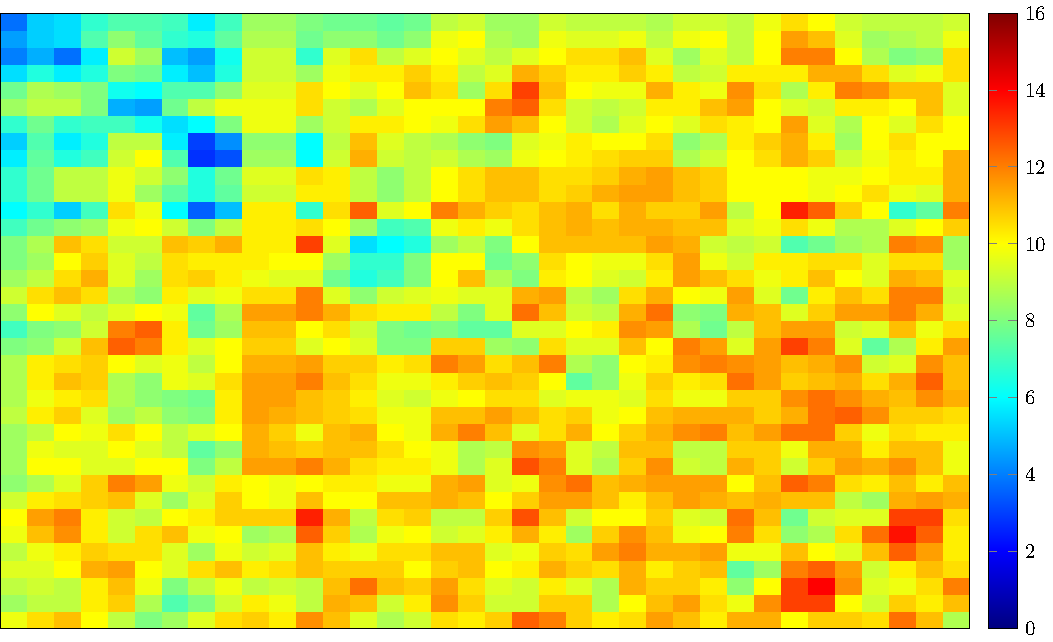
\includegraphics{figures/unknotting-moves-and-combinatorial-representations/mult-heatmap.pdf}
    \caption[Heatmap of Multiplication Table]{Heatmap for the
      multiplication table. Observe that the table is \emph{not}
      symmetric.}
    \label{tab:mult-heatmap}
  \end{figure}
\end{landscape}

\begin{landscape}
  \begin{figure}[H]
    \centering
    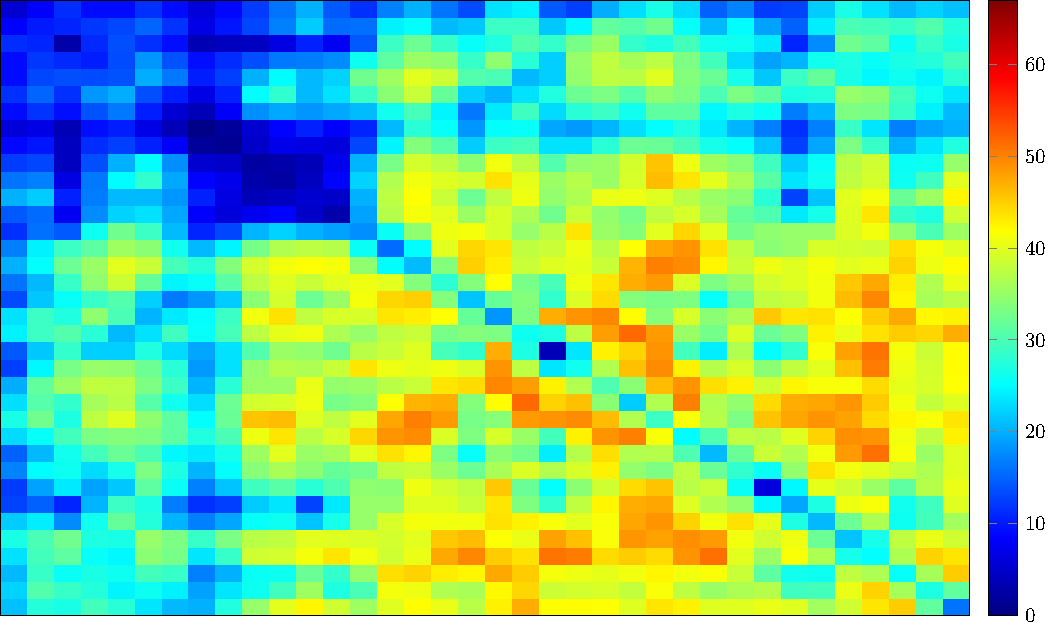
\includegraphics{figures/unknotting-moves-and-combinatorial-representations/po-heatmap.pdf}
    \caption[Heatmap of Pairwise Group Orders]{Log-scale heatmap
      showing the order of the group generated by pairs of our knot
      cycles. This one is symmetric.}
    \label{tab:po-heatmap}
  \end{figure}
\end{landscape}

%%% Local Variables:
%%% TeX-master: "../../kobayashi-thesis"
%%% End:
